\documentclass[a4paper,  11pt]{ctexart}
\usepackage{srcltx,graphicx}
\usepackage{amsmath, amssymb, amsthm}
\usepackage{color}
\usepackage{lscape}
\usepackage{multirow}
\usepackage{psfrag}
\usepackage{diagbox}
\usepackage[hang]{subfigure}
\usepackage{float}
\usepackage[colorlinks,linkcolor=black,anchorcolor=blue,citecolor=green]{hyperref}

\newtheorem{theorem}{Theorem}
\newtheorem{lemma}{Lemma}
\newtheorem{definition}{Definition}
\newtheorem{comment}{Comment}
\newtheorem{conjecture}{Conjecture}

\newcommand\bbR{\mathbb{R}}
\newcommand\bbN{\mathbb{N}}
\newcommand\bbC{\mathbb{C}}
\newcommand\bx{\boldsymbol{x}}
\newcommand\dd{\,\mathrm{d}}

\newcommand\diag{\mathrm{diag}}
\newcommand\tr{\mthrm{tr}}

\setlength{\oddsidemargin}{0cm}
\setlength{\evensidemargin}{0cm}
\setlength{\textwidth}{150mm}
\setlength{\textheight}{230mm}

\newcommand\note[2]{{{\bf #1}\color{red} [ {\it #2} ]}}
%\newcommand\note[2]{{ #1 }} % using this line in the formal version

\newcommand\pd[2]{\dfrac{\partial {#1}}{\partial {#2}}}
\newcommand\od[2]{\dfrac{\dd {#1}}{\dd {#2}}}
\newcommand{\bm}[1]{\mbox{\boldmath{$#1$}}}

\begin{document}
\title{图像处理中的数学方法—homework2}
\author{郑灵超}
\maketitle
% \tableofcontents
% \newpage

\section{理论分析}
将图像视为二维区域内的函数,作为PDE的初值,
则可以利用PDE来对图像进行去噪去模糊,利用如下形式的方程
\begin{equation*} 
	\left\{
	\begin{aligned}
		&\pd{u}{t}(t,x)+F(x,u(t,x),\nabla u(t,x),\nabla^2 u(t,x))
		=0\ \text{in}\ (0,T)\times \Omega, \\
		&\pd{u}{N}(t,x)=0 \ \text{on} (0,T)\times \partial\Omega, \\
		& u(0,x)=u_0(x).
	\end{aligned}
	\right.
\end{equation*}
其中常用的包括热方程,PM方程和shock-filter。
\subsection{热方程}
\begin{equation*}
	\left\{
	\begin{aligned}
	&\pd{u}{t}(t,x)-\nu\Delta u(t,x)=0, \ t \geq 0,\ x\in\bbR^2, \\
    &u(0,x)=u_0(x).
\end{aligned}
	\right.
\end{equation*}
为了求解此问题,我们采用如下的差分格式:
\[
v_{i,j}^{n+1}=v_{i,j}^n+\frac{\nu\Delta t}{h^2}
(v_{i+1,j}^n+v_{i-1,j}^n+v_{i,j+1}^n+v_{i,j-1}^n-4v_{i,j}^n).
\]
\subsection{PM方程}
\begin{equation*}
	\left\{
	\begin{aligned}
		&\pd{u}{t}(t,x)=\text{div}
		(c(|\nabla u(t,x)|^2)\nabla u(t,x)) \\
    &u(0,x)=u_0(x).
\end{aligned}
	\right.
\end{equation*}
即
\begin{equation*}
	\left\{
	\begin{aligned}
		&\pd{u}{t}(t,x)= c(|\nabla u(t,x)|^2)u_{TT}
		+b(|\nabla u(t,x)|^2)u_{NN}, \\
	&u(0,x)=u_0(x).
\end{aligned}
	\right.
\end{equation*}

此处$b(s)=c(s)+2sc'(s)$,一个常见的$c$的取法为
\[ c(s) = \frac{1}{\sqrt{1+s}}. \]

为了求解此问题,我们采用一个对称的差分格式
\[
   \text{div} (b\nabla v)|_{i,j} = \frac{1}{h^2}\left(
   b_{+0}v_{i+1,j}+b_{-0}v_{i-1,j}+b_{0+}v_{i,j+1}+b_{0-}v_{i,j-1}
   -(b_{+0}+b_{-0}+b_{0+}+b_{0-})v_{i,j} \right)
\]
其中
\[
b_{\pm 0}=b_{i\pm \frac12,j},\ b_{0\pm}=b_{i,j\pm\frac12}.
\]
\subsection{shock-filter}
\begin{equation*}
	\pd{u}{t}=-|\nabla u|F(L(u))
\end{equation*}
其中
\[ F(0)=0, \text{sign}(s)F(s)>0,\quad s\neq 0. \]
经典的$F(s)$的取法为
\[ L(u) = \Delta u =u_{xx}+u_{yy}, \]
一个更好的取法为
\[ L(u) = \frac{1}{|\nabla
u|^2}(u_x^2u_{xx}+2u_xu_yu_{xy}+u_y^2u_{yy}). 
\]

为了求解此问题,我们采用minmod限制器
\[
m(\alpha,\beta)=\left\{
\begin{aligned}
    &\text{sign}(\alpha)\text{min}(|\alpha|,|\beta|),\quad
    &\alpha\beta>0, \\
    &0, & \alpha\beta\leq 0.
\end{aligned}
\right.
\]
使用的数值格式为
\[
u_{i,j}^{n+1}=u_{i,j}^n-\frac{\Delta t}{h}\sqrt{
m(\delta_x^+u_{i,j}^n,\delta_x^-u_{i,j}^n)^2
+m(\delta_y^+u_{i,j}^n,\delta_y^-u_{i,j}^n)^2
}F_{i,j}(L(u^n)).
\]
其中 
\[
\delta_x^+v_{i,j}=\frac{1}{\Delta x}(v_{i+1,j}-v_{i,j}), \ 
\delta_x^-v_{i,j}=\frac{1}{\Delta x}(v_{i,j}-v_{i-1,j}),
\]
\[
\delta_y^+v_{i,j}=\frac{1}{\Delta y}(v_{i,j+1}-v_{i,j}), \ 
\delta_y^-v_{i,j}=\frac{1}{\Delta y}(v_{i,j}-v_{i,j-1}).
\]

\section{数值结果}
\subsection{热方程}
取参数$\nu=1,dt=0.01$,噪声为$\sigma \text{randn}$,对加噪后的图像
进行迭代,得到的误差随着迭代时间变化的结果如下:
\begin{figure}[H]
    \centering
    \subfigure{
    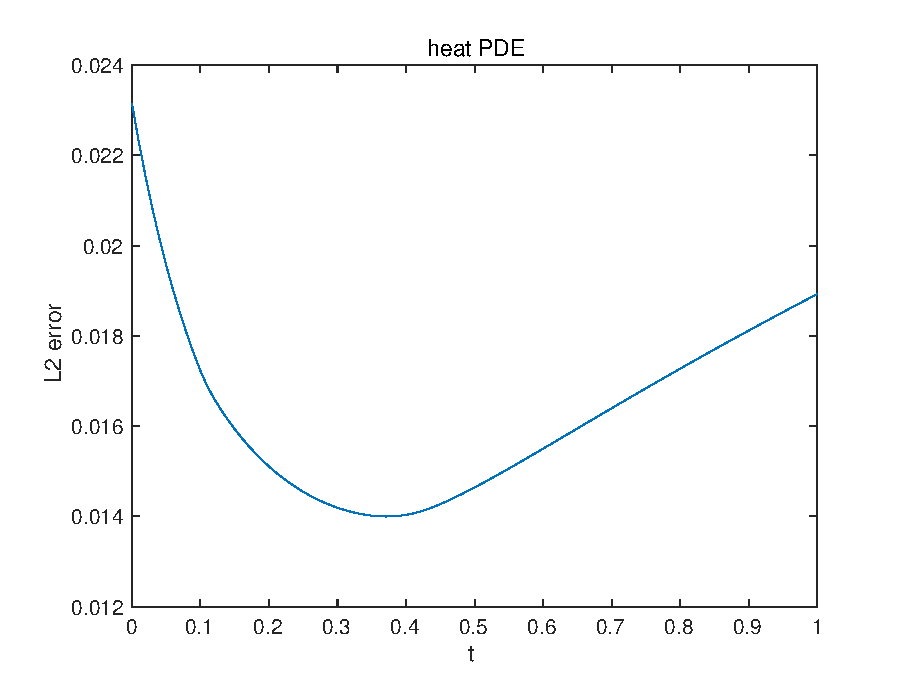
\includegraphics[width=0.45\textwidth]{../program/heaterr-1.eps}}
    \subfigure{
    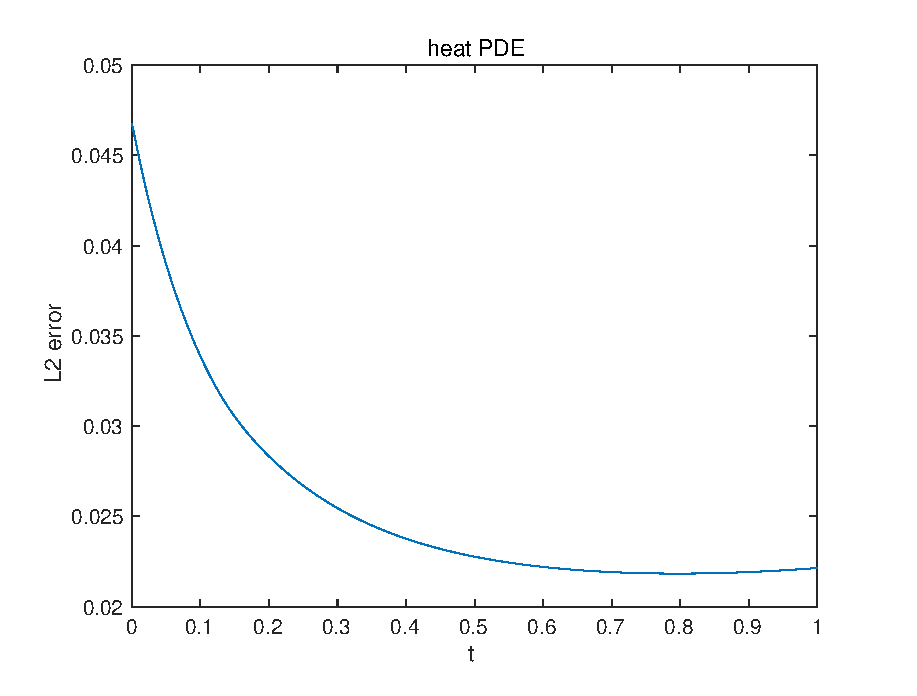
\includegraphics[width=0.45\textwidth]{../program/heaterr-2.eps}}
\end{figure}
其中左图$\sigma=\frac{\text{max}u}{10}$,右图
$\sigma=\frac{\text{max}u}{5}$。\par
左图迭代对应的结果图片为
\begin{figure}[H]
    \centering
    \subfigure[初始图片]{
    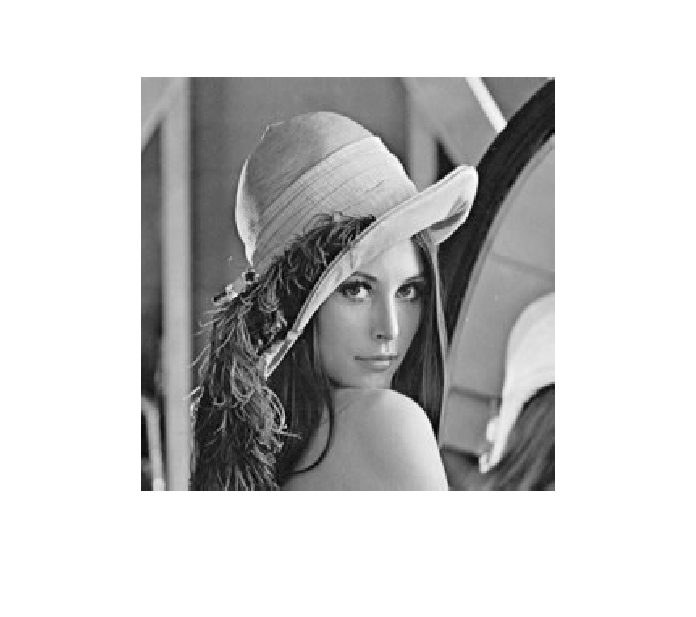
\includegraphics[width=0.45\textwidth]{../program/lenna.eps}}
    \subfigure[加噪图片]{
    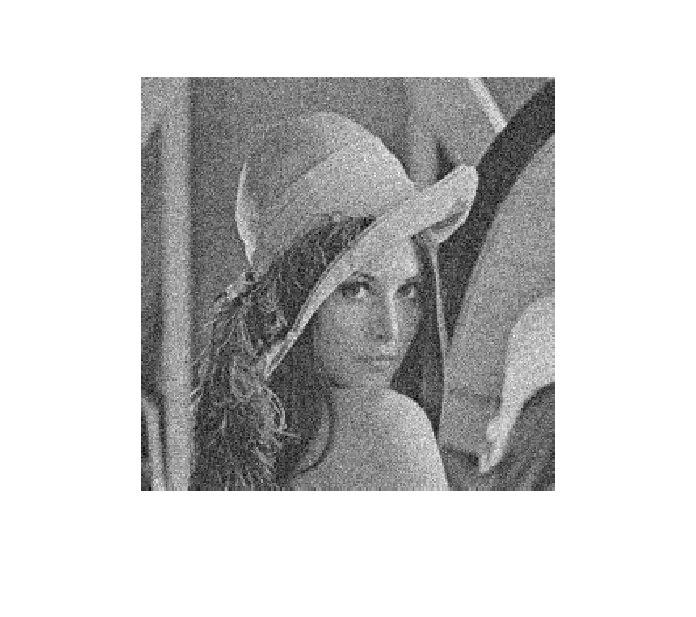
\includegraphics[width=0.45\textwidth]{../program/noise.eps}}
    \subfigure[去噪图片,t=0.3]{
    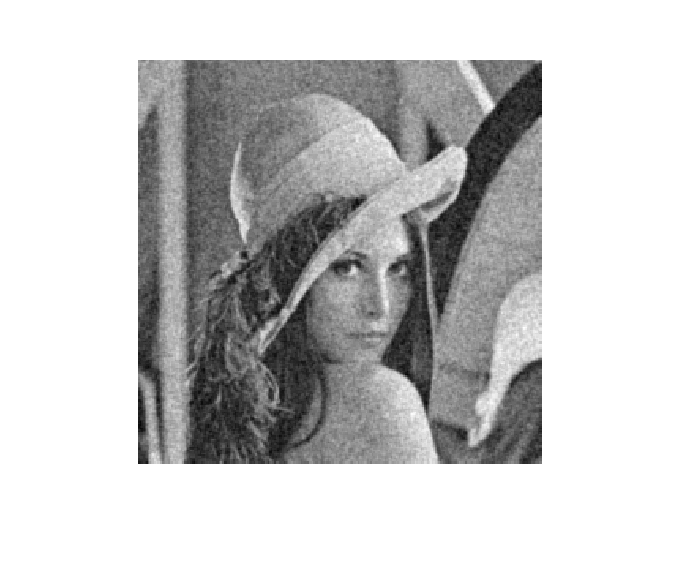
\includegraphics[width=0.45\textwidth]{../program/heat-1.eps}} 
    \subfigure[去噪图片,t=1]{
    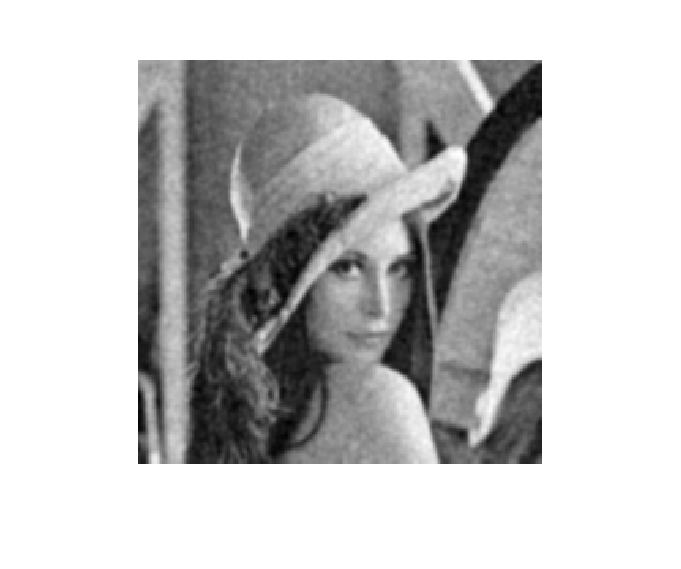
\includegraphics[width=0.45\textwidth]{../program/heat-2.eps}} 
\end{figure}
观察图片可以发现,随着迭代的进行,去噪效果会越来越明显,但热方程也会将
图片模糊化,随着时间的推进图片会趋于模糊,从而加大相对误差。
\subsection{PM方程}
和热方程相同,我们取参数$\nu=1,dt=0.01$,噪声为$\sigma \text{randn}$,对加噪后的图像
进行迭代,得到的误差随着迭代时间变化的结果如下:
\begin{figure}[H]
    \centering
    \subfigure{
    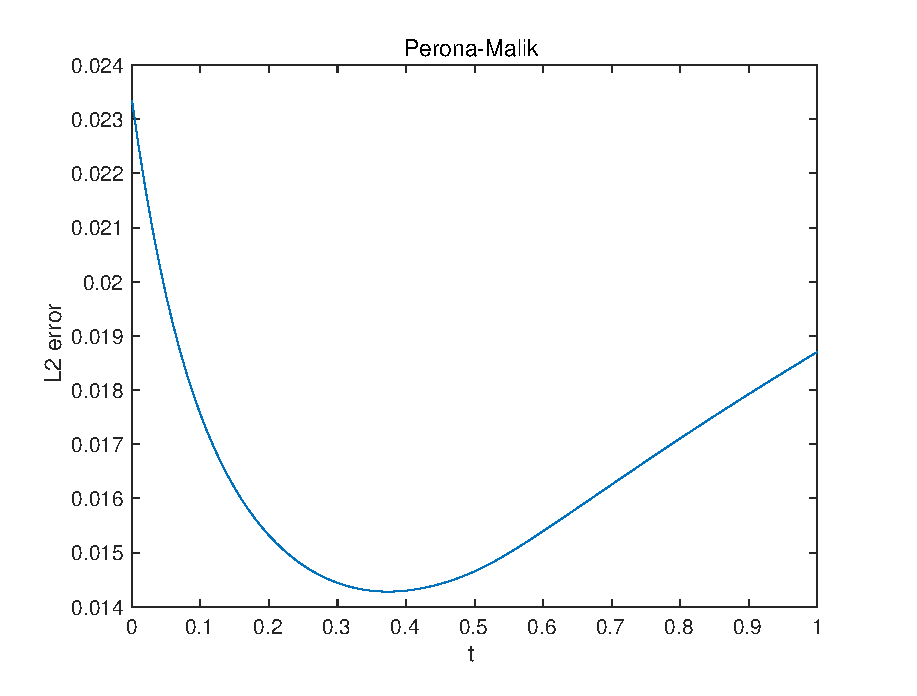
\includegraphics[width=0.45\textwidth]{../program/pmerr-1.eps}}
    \subfigure{
    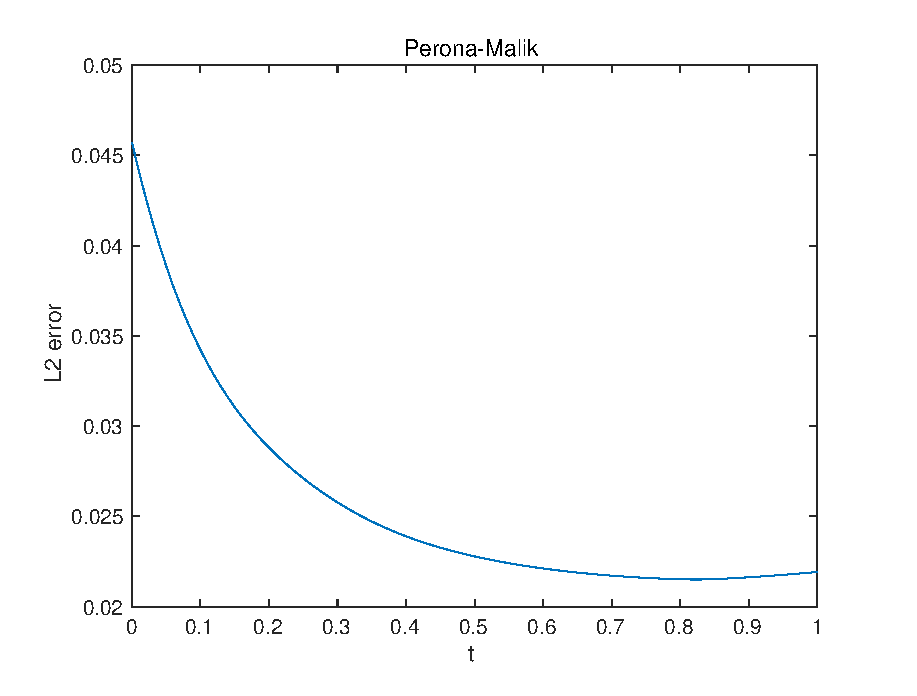
\includegraphics[width=0.45\textwidth]{../program/pmerr-2.eps}}
\end{figure}
其中左图$\sigma=\frac{\text{max}u}{10}$,右图
$\sigma=\frac{\text{max}u}{5}$。\par
左图迭代对应的结果图片为
\begin{figure}[H]
    \centering
    \subfigure[初始图片]{
    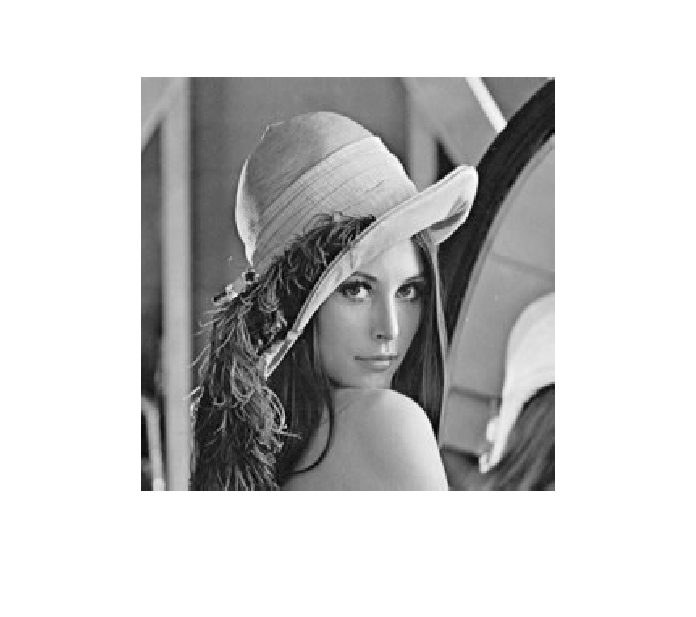
\includegraphics[width=0.45\textwidth]{../program/lenna.eps}}
    \subfigure[加噪图片]{
    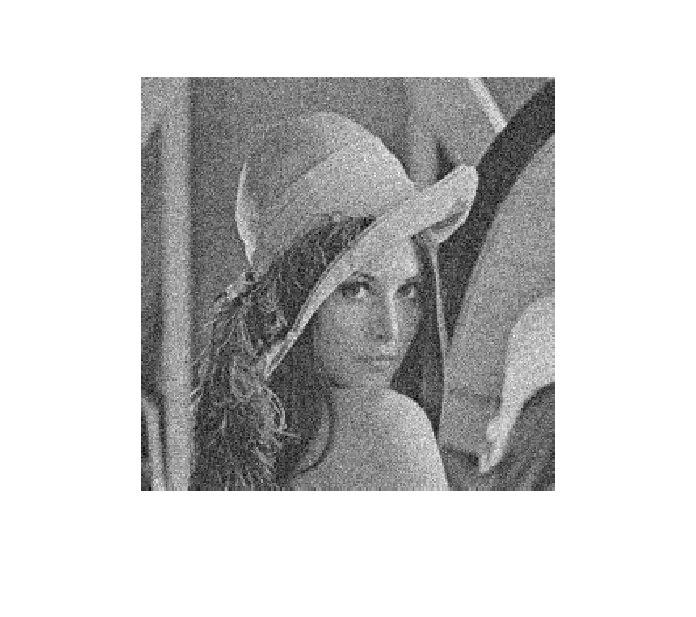
\includegraphics[width=0.45\textwidth]{../program/noise.eps}}
    \subfigure[去噪图片,t=0.4]{
    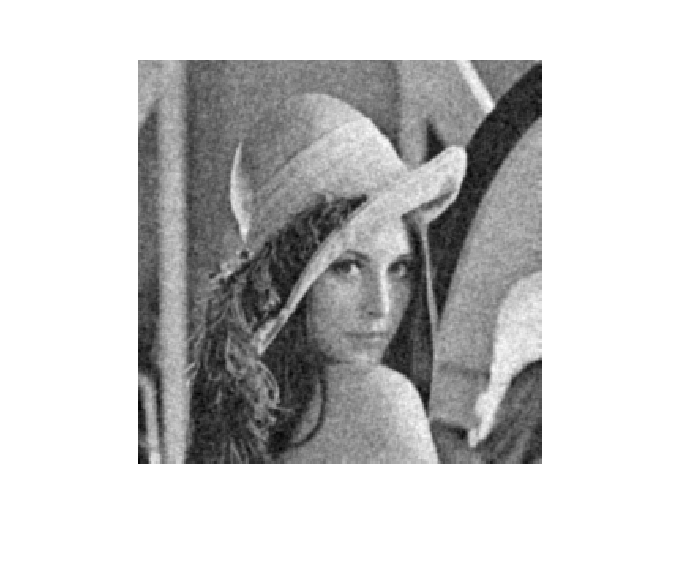
\includegraphics[width=0.45\textwidth]{../program/pm-1.eps}} 
    \subfigure[去噪图片,t=1]{
    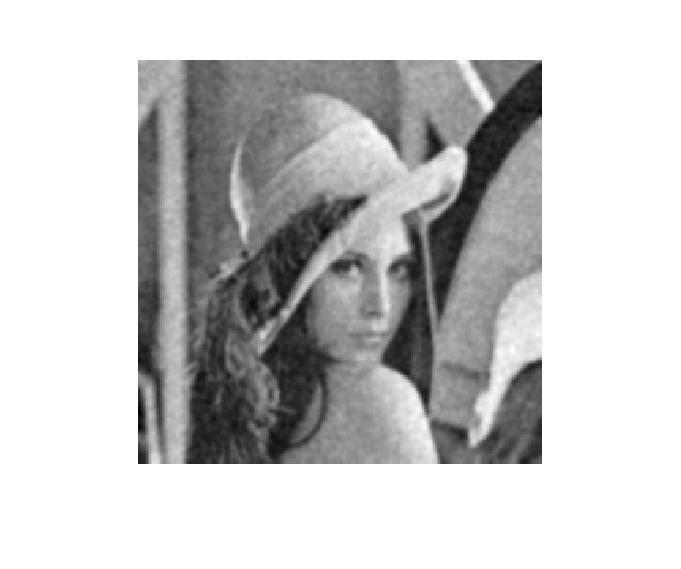
\includegraphics[width=0.45\textwidth]{../program/pm-2.eps}} 
\end{figure}
观察图片可以发现,随着迭代的进行,去噪效果会越来越明显,但PM方程也会将
图片模糊化,随着时间的推进图片会趋于模糊,从而加大相对误差。
\par
比较热方程和PM方程,可以发现二者性质类似,但总体而言热方程的去噪效果略
好一些。

\subsection{shock filters}
\subsubsection{不加噪声的去模糊}
我们采用对原图进行热方程迭代的方法来生成一个不加噪声的模糊图像,再用
shock-filters方法进行去模糊。\par
此处我们选取的参数$dt=0.1,T=30$,得到的结果如下:
\begin{figure}[H]
    \centering
    \subfigure[初始图片]{
    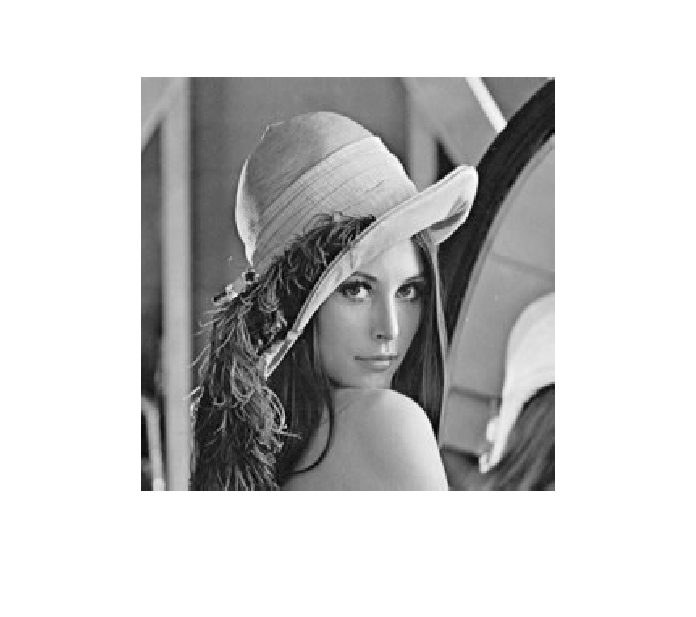
\includegraphics[width=0.45\textwidth]{../program/lenna.eps}}
    \subfigure[模糊图片]{
    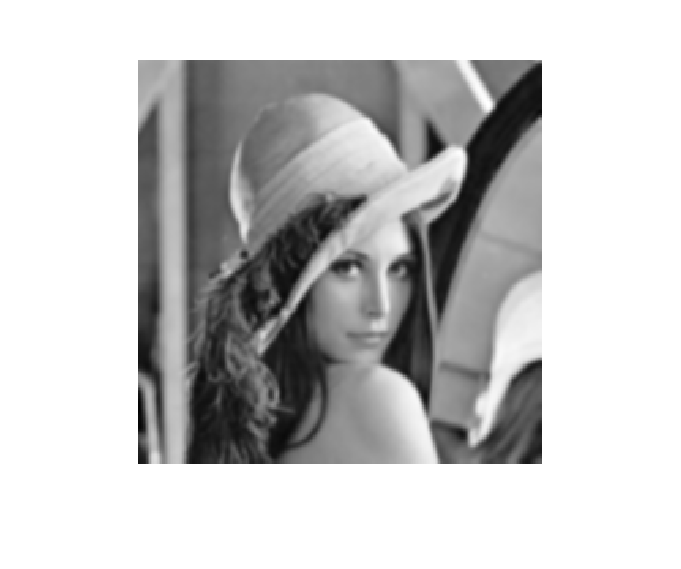
\includegraphics[width=0.45\textwidth]{../program/blurr.eps}}
    \subfigure[去模糊图片,采用L1]{
    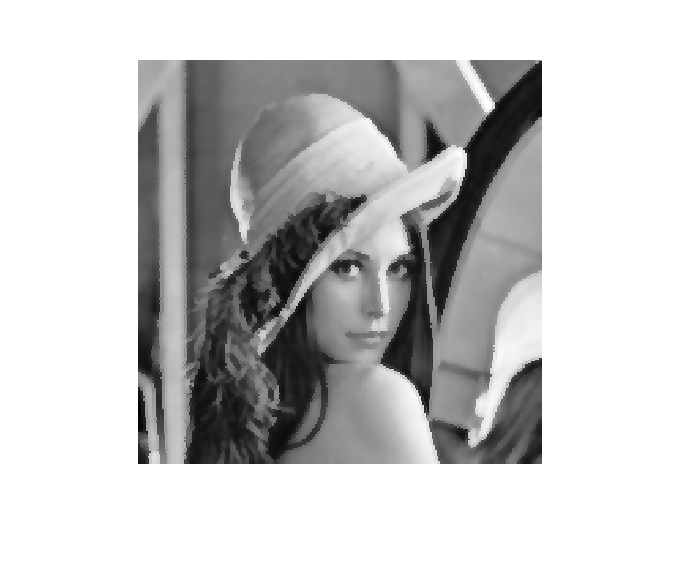
\includegraphics[width=0.45\textwidth]{../program/sf-1.eps}} 
    \subfigure[去模糊图片,采用L2]{
    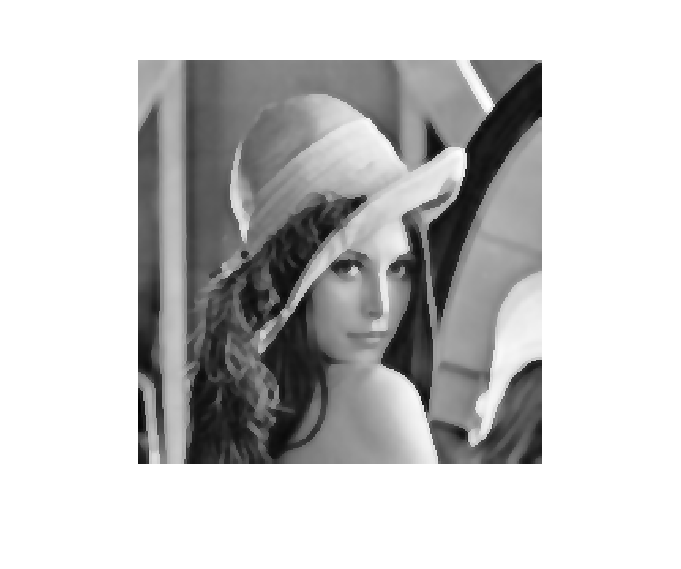
\includegraphics[width=0.45\textwidth]{../program/sf-2.eps}} 
\end{figure}
这里我们说的L1与L2分别表示
\[ L_1(u) = \Delta u =u_{xx}+u_{yy}, \]
\[ L_2(u) = \frac{1}{|\nabla
u|^2}(u_x^2u_{xx}+2u_xu_yu_{xy}+u_y^2u_{yy}). 
\]
误差随着迭代时间的变化情况如下图所示:
\begin{figure}[H]
    \centering
    \subfigure[采用L1]{
    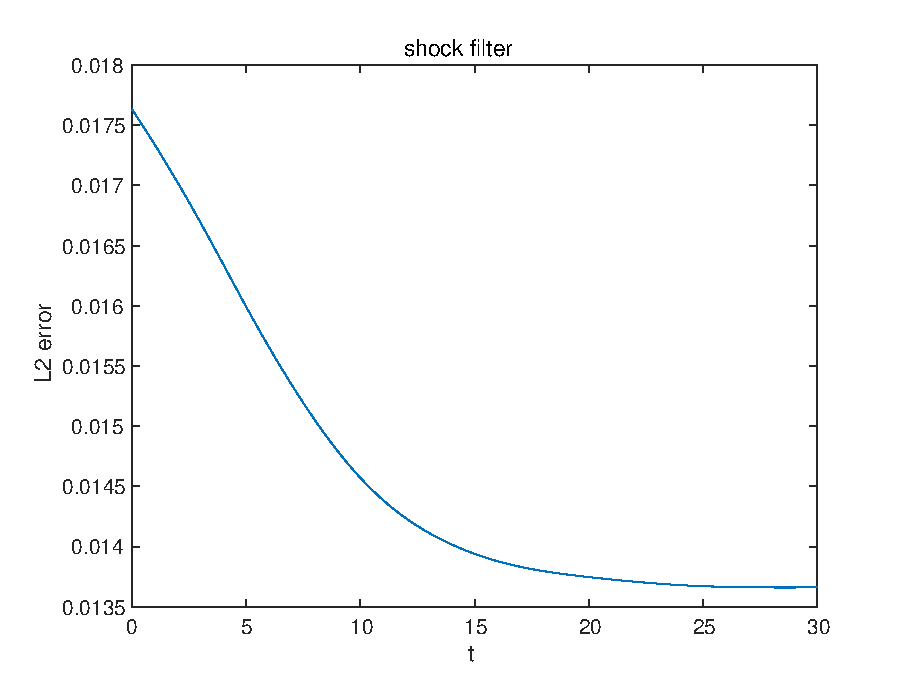
\includegraphics[width=0.45\textwidth]{../program/sferr-1.eps}}
    \subfigure[采用L2]{
    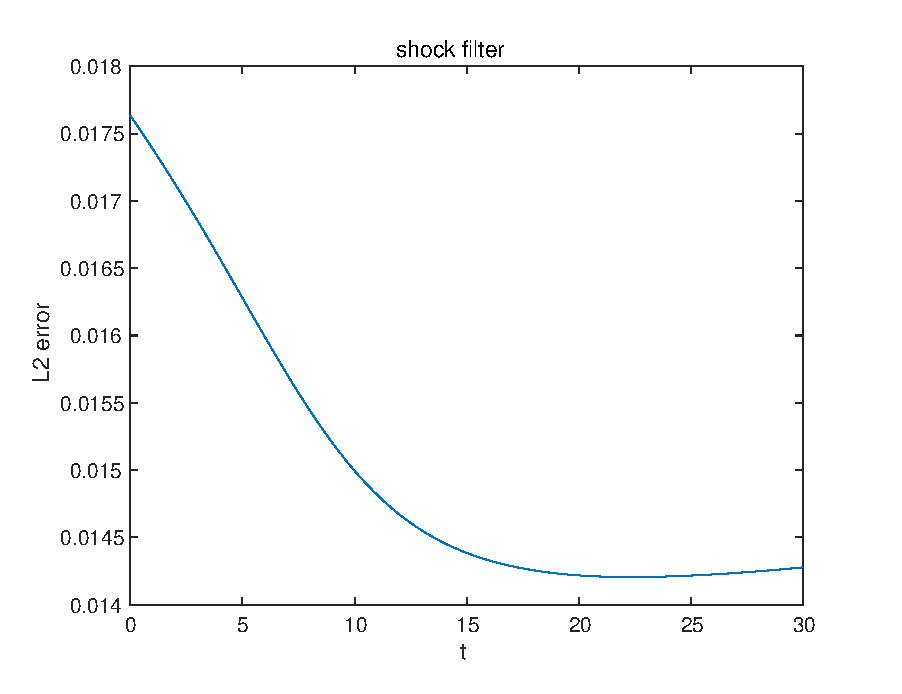
\includegraphics[width=0.45\textwidth]{../program/sferr-2.eps}}
\end{figure}

可以发现对没有噪声只有模糊的图片,shock-filters方法能够进行去模糊。
\subsubsection{加噪声的去模糊}
我们采用对加了噪声的图片进行热方程迭代,将所得结果作为模糊图像来让
shock-filters方法进行去模糊。
选取的参数与之前相同,$dt=0.1,T=30$,得到的结果如下:
\begin{figure}[H]
    \centering
    \subfigure[初始图片]{
    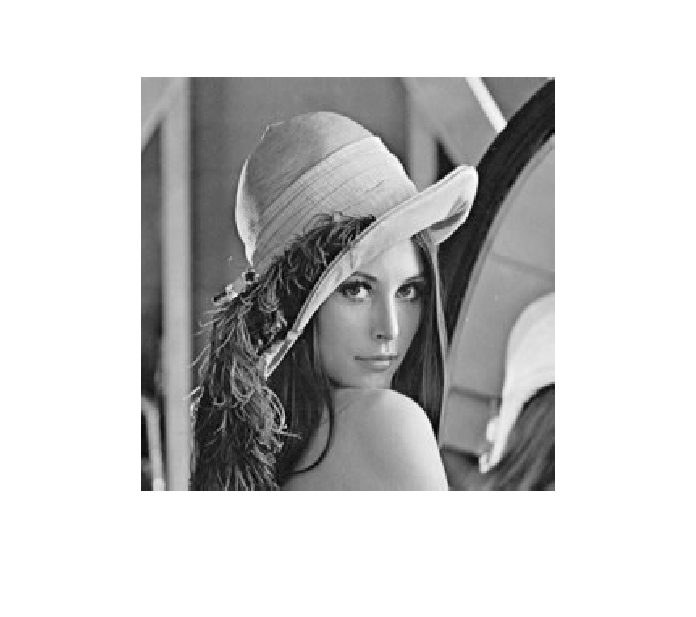
\includegraphics[width=0.45\textwidth]{../program/lenna.eps}}
    \subfigure[模糊图片]{
    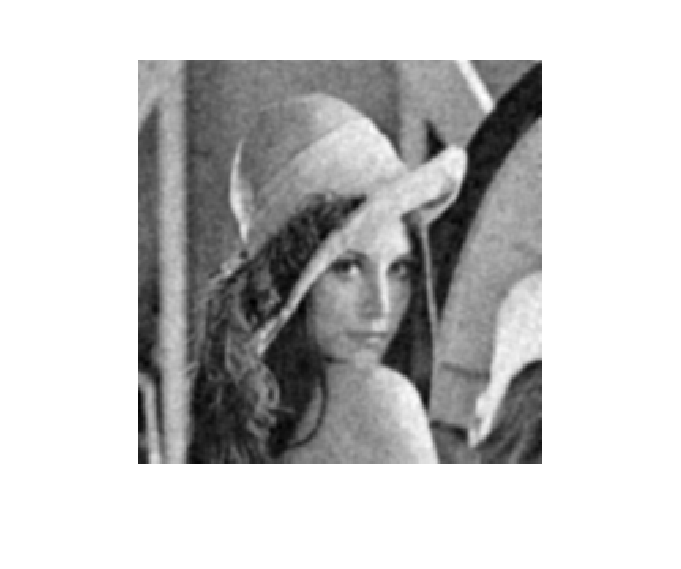
\includegraphics[width=0.45\textwidth]{../program/noise-blurr.eps}}
    \subfigure[去模糊图片,采用L1]{
    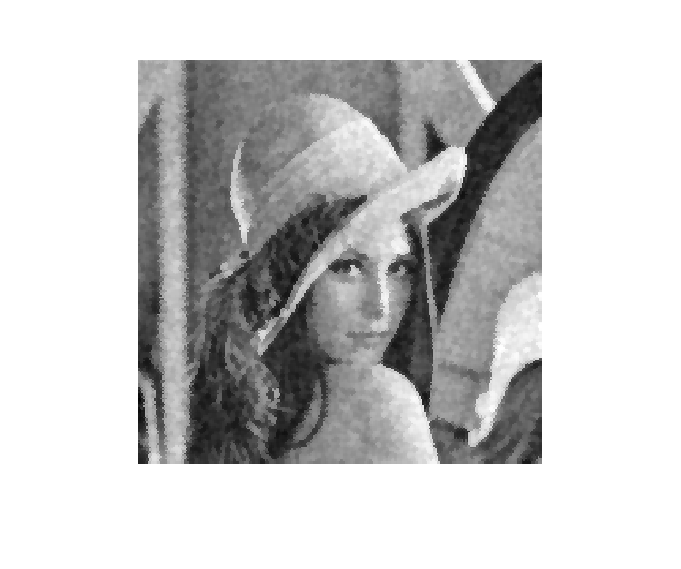
\includegraphics[width=0.45\textwidth]{../program/sf-3.eps}} 
    \subfigure[去模糊图片,采用L2]{
    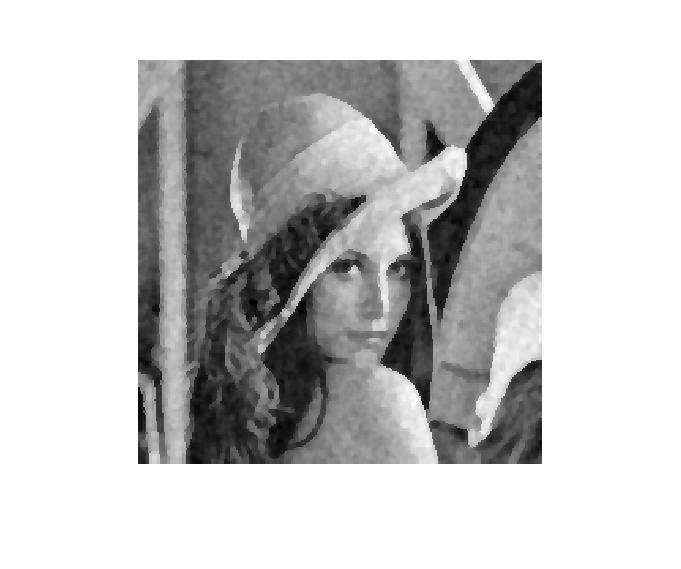
\includegraphics[width=0.45\textwidth]{../program/sf-4.eps}} 
\end{figure}
误差随着迭代时间的变化情况如下图所示:
\begin{figure}[H]
    \centering
    \subfigure[采用L1]{
    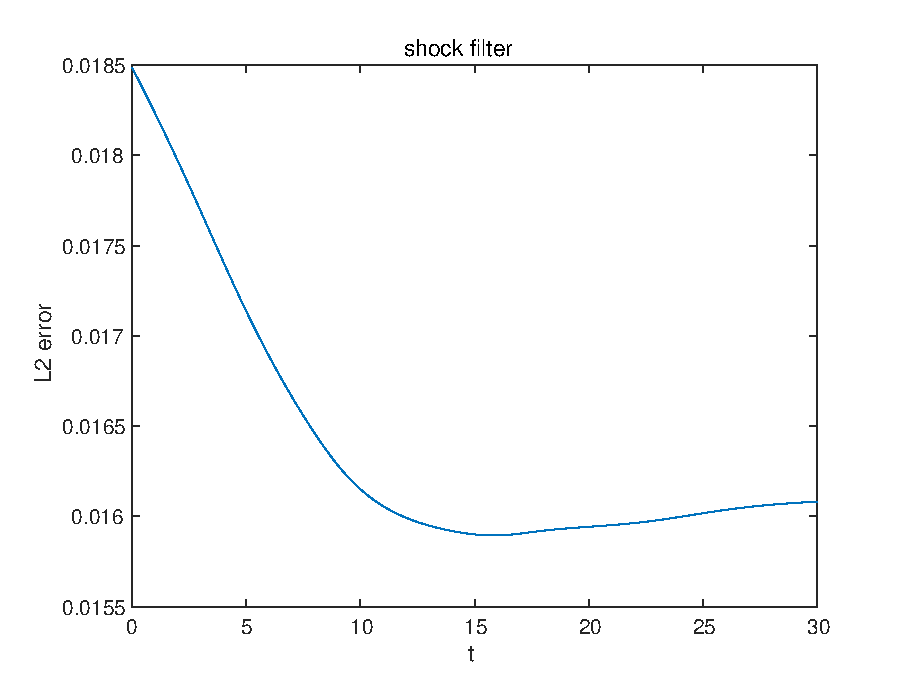
\includegraphics[width=0.45\textwidth]{../program/sferr-3.eps}}
    \subfigure[采用L2]{
    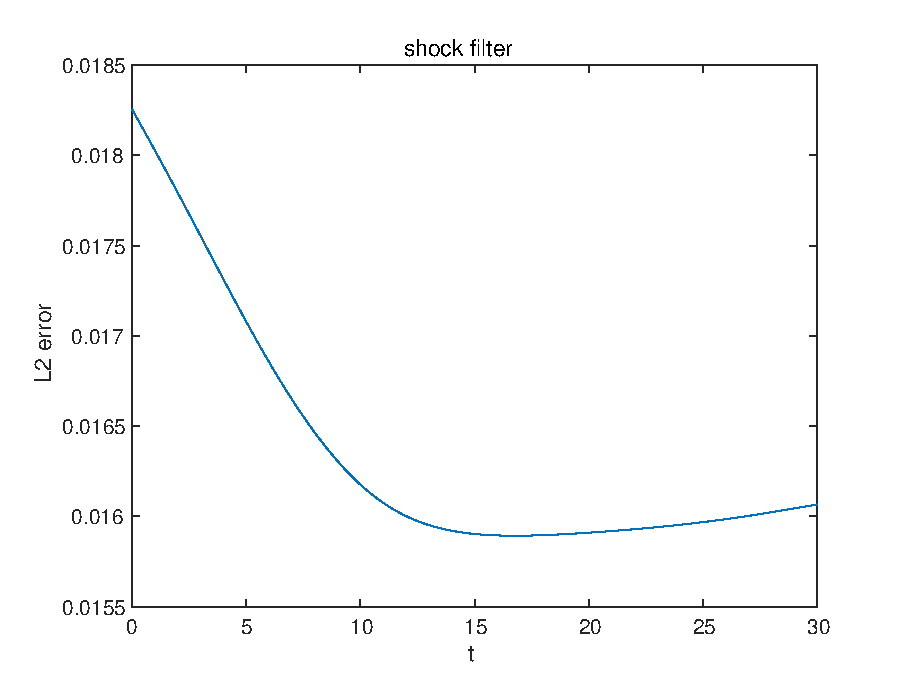
\includegraphics[width=0.45\textwidth]{../program/sferr-4.eps}}
\end{figure}
可见加了模糊之后,利用shock filters方法进行去模糊还有一定效果,
但作用降低了不少。

\section{上机报告总结}
本次图像处理作业我们利用了二维的偏微分方程,对图像进行了去噪和去模糊。
\par
我们采用了热方程和PM方程对图像进行去噪,它们是一个耗散的方程,能够将
图像中的噪声耗散从而进行去噪,但去噪的同时也将为图像引入模糊。
\par
shock filter方法可以用于去模糊,但经过实践表明,对于既有噪声又有模糊的
图像,该方法并不能取得太大的效果。

\end{document} 

